\documentclass[letterpaper, 10 pt, conference]{ieeeconf} 
\usepackage{ifpdf}
\usepackage{cite}
\usepackage{amsmath,bm}
\usepackage{amssymb}
\usepackage{algorithmic}
\usepackage{array}
\usepackage{url}
\usepackage{graphicx}
\usepackage{xcolor}
\usepackage{mathtools}
\usepackage{subfigure}
\usepackage{hyperref}
\newcommand{\RomanNumeralCaps}[1]
    {\MakeUppercase{\romannumeral #1}}

\IEEEoverridecommandlockouts       % This command is only needed if
                                    % you want to use the \thanks command
\overrideIEEEmargins                % Needed to meet printer requirements.
\newtheorem{rem}{Remark}
\setlength{\textfloatsep}{2.0pt plus 2.0pt minus 2.0pt}
\abovecaptionskip
\belowcaptionskip
\begin{document}
\title{ROS-Based \textbf{M}ulti-\textbf{A}gent \textbf{S}ystems \textbf{CO}ntrol Hybrid \textbf{T}estbed (MASCOT)}
\author{Arvind Pandit and Ameer K. Mulla\thanks{Arvind Pandit and Ameer K. Mulla are with the Department of Electrical Engineering, Indian Institute of Technology Dharwad, Karnataka, India. Email: \texttt{arvind.pandit.21@iitdh.ac.in, ameer@iitdh.ac.in}}}



%----------------- Title  ---------------------------------------
\maketitle
%-------------------Abstract and Keywords----------------------------
\begin{abstract}
    This paper presents a hybrid multiagent system simulation testbed with human in the loop control which is developed for testing and demonstration of different linear and non-linear decentralized control algorithms designed for multiagent system.This paper is aimed at the development of the platform which bridges a gap between theory and practical for the deployment of such algorithms. This platform supports Human in loop control where the leader are bilaterally teleoperated using a 3-DOF Novint Falcon haptic controller. The system developed provides the testbed for the simulation of multiagent systems having quadcopter agents. Here the quadcopter are assummed to have a simple dynamics as a simple and double integrator system. This is based on the fact that under certain assumptions, quadcopter dynamics can be  modeled as a double integrator system. There is also hybrid simulation structure in the platform which enables user to simulate agents a mixture of virtual and real agents. Crazyflie 2.1 is used a hardware agent for the hybrid simulation. A gazebo simulator with a physics engine as ODE (Open Dynamics Engine) is used for simulating the dynamics of the quadcopter. Robot Operating System is used to develop communication networks and motion control algorithms for the different agents in the simulation testbed. The performance of the test bed is analyzed by implementing linear control laws such as position control, leaderless consensus, leader-follower consensus, bearing based formation and non-linear control law for min-max time consensus. This work is published as an open-source ROS package under MIT license at \url{https://github.com/Avi241/mascot}. A docker image is also developed for easy setup of the system.
\end{abstract}
% % Note that keywords are not normally used for peer review papers.
% \begin{keywords}
% Multi-Agent Systems, Simulation Test-bed, ROS, Gazebo
% \end{keywords}


%---------------- Introduction -----------------------------------------
\section{Introduction}



%\textit{Notations:}

%---------------- Preliminaries -----------------------------------------

\section{Preliminaries}\label{sec:prelim}
In this section, first, we describe the preliminaries of the dynamics of a quadcopter and review how a quadcopter can be represented using double integrator dynamics. A few preliminaries used in distributed control of multi-agent systems are also discussed.
\subsection{Frame of References}\label{subsec:for}
Figure \ref{Fig: Quad Dynamics} shows the standard definitions \cite{Robotics_Vision_Control} of the reference frames used in this simulation. $\{E\}$ is the \textit{Earth reference frame} having its $z$-axis facing upward in the space. The body coordinate frame, $\{B\}$ is attached to the center of the quadcopter having its $z$-axis facing downwards in the space. $\{B^{\prime}\}$ reference frame is attached to the body having its origin same as $\{B\}$ and $x^{B^{\prime}}y^{B^{\prime}}$ plane is parallel to $x^{E}y^{E}$.

\begin{figure}[!ht]
    \centering
    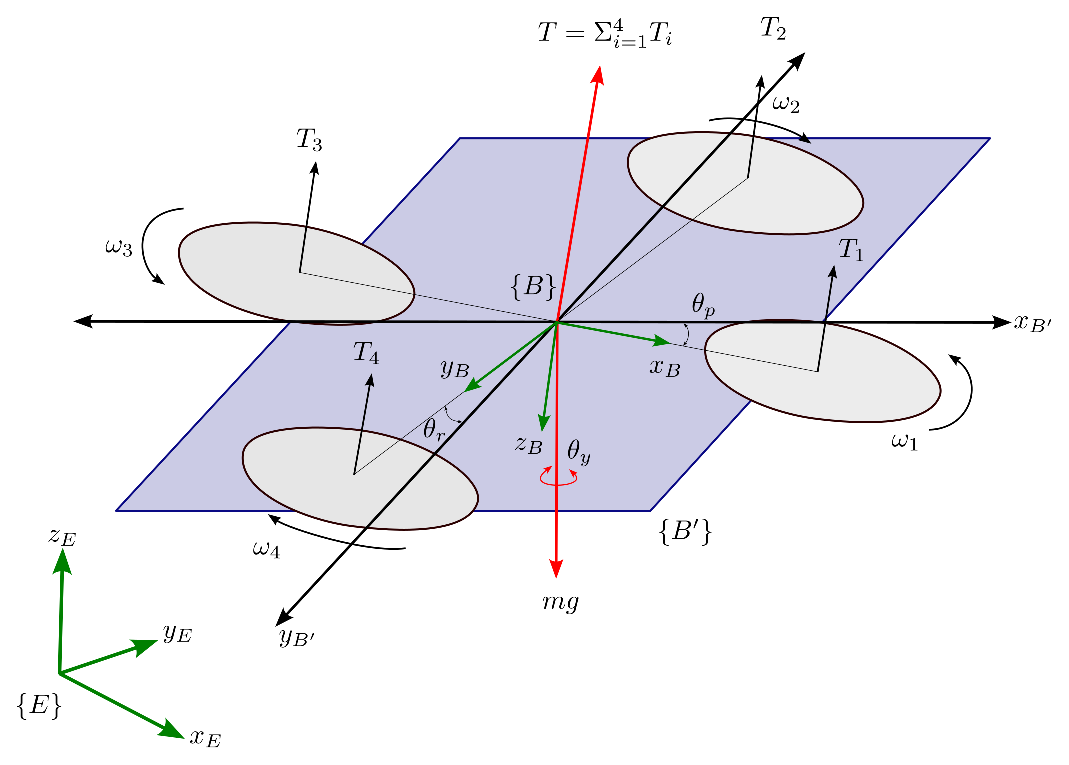
\includegraphics[scale=0.40]{Quadcopter.eps}
    \caption{Quadcopter reference frames setup}
    \label{Fig: Quad Dynamics}
\end{figure}
The angles $\theta_{p}$ (pitch), $\theta_{r}$ (roll), and $\theta_{y}$ (yaw) represents the rotation of the body along $x$, $y$, and $z$-axis of the reference frame respectively. As $x^{B^{\prime}}y^{B^{\prime}}$ plane is parallel to $x^{E}y^{E}$ thus $\{B^{\prime}\}$ can only rotate along the z-axis with angle $\theta_{p}$. The change in orientation between $\{B^{\prime}\}$ and \{E\} is given by a rotation matrix
\begin{equation*}
    \mathbf{R}_{B^{\prime}}^{E}=\begin{bmatrix}
        c \theta_{y}  & s \theta_{y} & 0 \\
        -s \theta_{y} & c \theta_{y} & 0 \\
        0             & 0            & 1
    \end{bmatrix}
\end{equation*}
where $ c(.) \coloneqq \cos{(.)} $ and $ s(.) \coloneqq \sin{(.)}$

\subsection{Quadcopter Dynamics}\label{subsec:qd}
The upward thrust along the $-z^{B}$ axis is given by
\begin{equation*}
    T_{i} = b\bar{\omega}_{i}^2
\end{equation*}
where $\omega_{i}$ is the angular velocity of the rotor and $b>0$ is a lift constant that depends on the air density, number of blades, cube of rotor blade radius, and chord length of the blade.
According to Newton's second law of motion, the translation dynamics of the quadcopter in $\{E\}$ is given by
\begin{equation}
    m\dot{\mathbf{v}}^{E}=\begin{bmatrix}
        0 & 0 & m g
    \end{bmatrix}^{T}-\mathbf{R}_{B}^{E}\begin{bmatrix}
        0 & 0 & T
    \end{bmatrix}^{T} - B\mathbf{v}\label{eq:trans_dynamics}
\end{equation}
where $\mathbf{v}$ is the velocity of quadcopter in \{E\} given by $\mathbf{v} =\begin{bmatrix}  {v_{x}}^{E} & {v_{y}}^{E} & {v_{z}}^{E} \end{bmatrix}^{T} \in \mathbb{R}^{3}$ , $B$ is aerodynamics friction and  $T = \Sigma T_{i}$ is total upward thrust generated by the rotors in $-z^{B}$ direction, $g$ is the gravitational acceleration, and $m$ is the mass of quadcopter. In \eqref{eq:trans_dynamics}, first term represents the gravitational force acting in $-z^{E}$ direction, second term represents the total upward thrust generated in  $-z^{B}$ direction in $\{B\}$ and rotated in $\{E\}$.

The rotation in each axis is obtained by varying pairwise differences in rotor thrust. Torque about $x$ and $y$ axes is given by
\begin{equation*}
    \tau_{x}=d T_{4}-d T_{2} = db(\bar{\omega}_{4}^{2}-\bar{\omega}_{2}^{2})
\end{equation*}
\begin{equation*}
    \tau_{y}=d T_{1}-d T_{3} = db(\bar{\omega}_{1}^{2}-\bar{\omega}_{3}^{2})
\end{equation*}
The torque applied to each motor is opposed by aerodynamic drag and exerts a reaction torque on the frame which is given by $Q_{i}=k\bar{\omega}_{i}$ where $k$ depends on the same factors as $b$.
The total reaction torque about $z$-axis is given by
\begin{equation}
    \tau_{z} =Q_{1}-Q_{2}+Q_{3}-Q_{4}=k\left(\bar{\omega}_{1}^{2}+\bar{\omega}_{3}^{2}-\bar{\omega}_{2}^{2}-\bar{\omega}_{4}^{2}\right)\label{eq:react_torque_z}
\end{equation}

The total torque applied to the quadcopter body is  $ \mathbf{\Gamma} =\begin{bmatrix}  {\tau}_{x} & {\tau}_{y} & {\tau}_{z} \end{bmatrix}$. By Euler's equation of motion rotational acceleration is given is by
\begin{equation}
    J\boldsymbol{\Dot{\omega}}=-\boldsymbol{\omega} \boldsymbol{\times}J \boldsymbol{\omega}+\mathbf{\Gamma}
\end{equation}
where J is the $3\times3$ inertia matrix of the quadcopter and $\omega$ is a angular velocity vector of the quadcopter body frame.
Overall quadcopter motion equation \cite{Robotics_Vision_Control} is obtained by integrating equations \eqref{eq:trans_dynamics} and \eqref{eq:react_torque_z} which is given by
\begin{align}
    \begin{bmatrix}
        \mathbf{T} &
        \mathbf{\Gamma}
    \end{bmatrix}^T & =A\begin{bmatrix}
        \bar{\omega}_{1}^{2} &
        \bar{\omega}_{2}^{2} &
        \bar{\omega}_{3}^{2} &
        \bar{\omega}_{4}^{2}
    \end{bmatrix}^T
\end{align}

\noindent where $A =\begin{bmatrix}
        -b  & -b   & -b   & -b  \\
        0   & -d b & 0    & d b \\
        d b & 0    & -d b & 0   \\
        k   & -k   & k    & -k
    \end{bmatrix}$ is a constant invertible matrix since $b,k,d > 0$.
%Thus A can be inverted to get the rotor speed given thrust and torque.
%\begin{equation}
%\begin{bmatrix}
%\bar{\omega}_{1}^{2} & \bar{\omega}_{2}^{2} & \bar{\omega}_{3}^{2} & \bar{\omega}_{4}^{2}
%\end{bmatrix}^{T}=A^{-1}\begin{bmatrix}
%\mathbf{T} & \mathbf{\Gamma}
%\end{bmatrix}^{T}
%\end{equation}

\subsection{Quadcopter Dynamics as Double Integrators}\label{subsec:di}

%All the actuators in the real world generated the force or torque which is used to run any system thus modeling any system that can be controlled by a force command reduces the complexity of the system and also eliminates the need for intermediate controllers such as velocity controller in this case of the quadcopter, which reduces the computation load.

The overall motion in the plane $x^{B^{\prime}}y^{B^{\prime}}$ is obtained by pitching and rolling the quadcopter by an angle $\theta_{p}$ and $\theta_{r}$. The total force acting on a quadcopter is given by
\begin{equation}
    \mathbf{f}^{B^{\prime}}=\mathbf{R}{x}\left(\theta{r}\right) \mathbf{R}{y}\left(\theta{p}\right)\begin{bmatrix}
        0 & 0 & T
    \end{bmatrix}^{T}\label{eq:total_force}
\end{equation}
where,
\begin{align*}
    \mathbf{R}{x}\left(\theta{r}\right)=\begin{bmatrix}
        1 & 0             & 0            \\
        0 & c \theta_{r}  & s \theta_{r} \\
        0 & -s \theta_{r} & c \theta_{r}
    \end{bmatrix},
    ~
    \mathbf{R}{y}\left(\theta{p}\right)=\begin{bmatrix}
        c \theta_{p}  & 0 & s \theta_{p} \\
        0             & 1 & 0            \\
        -s \theta_{p} & 0 & c \theta_{p}
    \end{bmatrix}
\end{align*}
are the Rotation matrix about $x$ and $y$ axes respectively.\\
Simplifying \eqref{eq:total_force} we get $\mathbf{f}^{B^{\prime}}$ as
\begin{equation*}
    \mathbf{f}^{B^{\prime}}=\begin{bmatrix}
        T\sin{\theta_{p}} & T\sin{\theta_{r}}\cos{\theta_{p}} & T\cos{\theta_{r}}\cos{\theta_{p}}
    \end{bmatrix}^{T}
\end{equation*}
for small $\theta_{p}$ and $\theta_{r}$ the above equation can be approximated by
\begin{equation*}
    \mathbf{f}^{B^{\prime}} \approx \begin{bmatrix}
        T\theta_{p} & T\theta_{r} & T
    \end{bmatrix}^{T}
\end{equation*}
i.e $f_{x}^{B^{\prime}} \approx T\theta_{p}$ and $f_{y}^{B^{\prime}} \approx T\theta_{r}$ \\
According to Newton's Second law of motion $F=ma$, we can write
\begin{equation*}
    ma_{x}^{B^{\prime}} = T\theta_{p}
\end{equation*}
\begin{equation*}
    \theta_{p} = \dfrac{m}{T}a_{x}^{B^{\prime}},~~\theta_{r} = \dfrac{m}{T}a_{y}^{B^{\prime}}
\end{equation*}
% Similarly for $\theta_{r}$,
% \begin{equation*}
%     \theta_{r} = \dfrac{m}{T}a_{y}^{B^{\prime}}
% \end{equation*}
where $a_{x}^{B^{\prime}}$ is  $a_{y}^{B^{\prime}}$ is acceleration of quadcopter in $\{B^{\prime}\}$ frame.\\
As the controller will receive the position and velocity in $\{E\}$ frame so it will compute the acceleration in $\{E\}$ frame which needs to be rotated to the $\{B^{\prime}\}$ frame.
\begin{equation*}
    \mathbf{f}^{B^{\prime}} = \mathbf{R}_{E}^{B^{\prime}}\mathbf{f^{E}}
\end{equation*}
\begin{equation*}
    m\mathbf{a}^{B^{\prime}} = \mathbf{R}_{E}^{B^{\prime}}m\mathbf{a^{E}}
\end{equation*}
\begin{equation*}
    \mathbf{a}^{B^{\prime}} = \mathbf{R}_{E}^{B^{\prime}}\mathbf{a^{E}}
\end{equation*}

This equation shows the motion of the quadcopter in $x^{B^{\prime}}y^{B^{\prime}}$ plane.

\begin{rem}
    While the discussion above describes the motion of the quadcopter in $x^{B^{\prime}}y^{B^{\prime}}$ plane as a double integrator, motion along $-z^{B^\prime}$ is directly dependent on the thrust generated by the rotors in \{B\} frame given by $T = \Sigma T_{i}$, which is naturally a double integrator.
\end{rem}

\subsection{Preliminaries of Distributed Control}
A homogeneous multi-agent system is a collection of $n$ agents with identical dynamics communicating with each other over a communication graph $\mathcal{G}=(\mathcal{V}, \mathcal{E})$, where the set of vertices $\mathcal{V}=\{\alpha_i,~i=1,...,n\}$ represents the agents and the edges $(\alpha_i,\alpha_j)\in\mathcal{E}$ denote the communication from agent $\alpha_i$ to $\alpha_j$. The communication graph $\mathcal{G}$ is \textit{undirected} if $(\alpha_i,\alpha_j)\in\mathcal{E}\implies(\alpha_j,\alpha_i)\in\mathcal{E}$
otherwise it is \textit{directed}. A \textit{path} in a graph is a sequence of edges. An undirected graph is said to be \textit{connected} if it has a path from each agent to every other agent. A directed graph is said to contain a \textit{directed spanning tree} if there is an agent $\alpha_r$ (called \textit{root}) such that there is a directed path from $\alpha_r$ to every other agent. Set of neighbours for each agent is given by $\mathcal{N}_{i} := \{j \in \mathcal{V} : (\alpha_i,\alpha_j) \in \mathcal{E} \}$. The Laplacian matrix $\mathcal{L}$ of a graph $\mathcal{G}$ is given by $\mathcal{L}_{n}=\left[l{i j}\right] \in \mathbb{R}^{n \times n} ; l_{i j}=-a_{i j}, i \neq j, l_{i i}=\sum_{j=1, j \neq i}^{n} a_{i j} $, where $a_{ij}$ is the \textit{weight} of the edge $(\alpha_i, \alpha_j)$.
Some control algorithms use leader-follower configuration of the multi-agent systems in which, the set of agents is divided into a set of leader $\mathbf{L}$ and a set of followers $\mathbf{F}$.

In this paper, agents are assumed to have double-integrator dynamics, given by
\begin{equation}
    \ddot{\mathbf{x}}_i^E(t)=\mathbf{f}_i^E(t)\label{eq:agent}
\end{equation}
\noindent where $\mathbf{x}_i^E=\begin{bmatrix}\mathbf{p}^E_i\\\mathbf{v}^E_i\end{bmatrix}\in\mathbb{R}^{2d}$ is the state vector of $\alpha_i$ and $\mathbf{f}^E_i\in\mathbb{R}^d$ denotes the input to $\alpha_i$. The vectors $\mathbf{p}^E_i$ and $\mathbf{v}^E_i$ denote the position and velocity of $\alpha_i$, respectively, in $\{E\}$ frame.
\begin{equation}
    f_{i}^{E}=\left\{\begin{array}{l}
        \sum_{j = 1}^{n} %a_{ij}\left(\mathbf{p}{j}^{E}-\mathbf{p}{i}^{E}\right)-\beta %v_{i}^{E} \text { if } a_{i} \in \mathcal{B} \\
        \\
        0 \text { if }  a_{i} \in \mathcal{A}
    \end{array}\right.
\end{equation}
where $a_{ij}$ is the (i,j) entry of the adjacency matrix $A_{n} \in \mathbb{R}^{n \times n}$ corresponding to the communication graph $\mathcal{G}_{n}$ and $\beta$ is a positive constant.This control law is the modified version of the control law mentioned in \cite{Distributed_Consensus_book}.The derivation of this law is provided in \cite{implementation_of_distributed_consensus}.The leader position is seprately controlled by a waypoint Navigation Controller.The control law discussed here drives \textbf{n} quadcopters to consensus i.e for any initial $p_{i}^{E}$ and $v_{i}^{E}$ and for all i,j = 1,....,n i.e $||p_{i}^{E}(t)-p_{j}^{E}(t)||\rightarrow0$ and $v_{i}^{E}(t)\rightarrow0$ as $t\rightarrow \infty$.

\begin{rem}
    The heading control loop given in the next section is designed such that $\theta_{y} \rightarrow \theta_{y}^{*}$ relatively fast and is held constant. Thus, matrix $\mathbf{R}_{B^{\prime}}^{E}$ can be considered as constant.
\end{rem}

\subsection{Preliminaries of Bearing based Formation Control}

\subsection{Preliminaries of Human-in-the-loop Control}
Human-in-the-loop (HITL) refers to a type of system in which a human operator is involved in the control loop of a robotic system. In a robotics simulator, human-in-the-loop typically means that a human operator can interact with the simulated robotic system in real time and make decisions or provide input that affects the behavior of the simulated robot.
\begin{figure}[!ht]
    \centering
    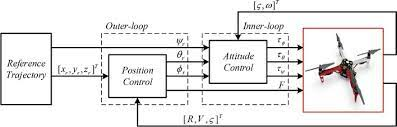
\includegraphics[scale=0.60]{HITL.jpeg}
    \caption{Human-in-the-loop control Block diagram}
    \label{Fig: HITL}
\end{figure}
There are many potential applications for human-in-the-loop robotics simulations. For example, a robotics simulator with human-in-the-loop functionality could be used to test and evaluate the performance of a new robotic system, or to train operators to work with the system in a safe and controlled environment. It could also be used to test and validate control algorithms or other software that will be used to operate the real-world robotic system.





\section{MASCOT: Structure and Features}\label{sec:mascot}



\subsection{Tools Used}\label{subsec:tools}
\subsubsection{Robot Operating System (ROS)}
ROS is an open-source framework that helps researchers and developers build and reuse code between robotics applications. ROS provides a distributive architecture that eliminates the problem of a single node handling all the tasks. ROS supports low-level drivers and programming in various languages such as Python, C++, Java, and Lisp. This makes it convenient to directly deploy the codes written for simulation on the physical systems. Visualization and debugging tools such as Rviz and rqt make it very easy to keep track of the process\cite{ros}. The basic architecture of ROS is shown in Fig. \ref{Fig:ROS Architecture}.
\begin{figure}[!ht]
    \centering
    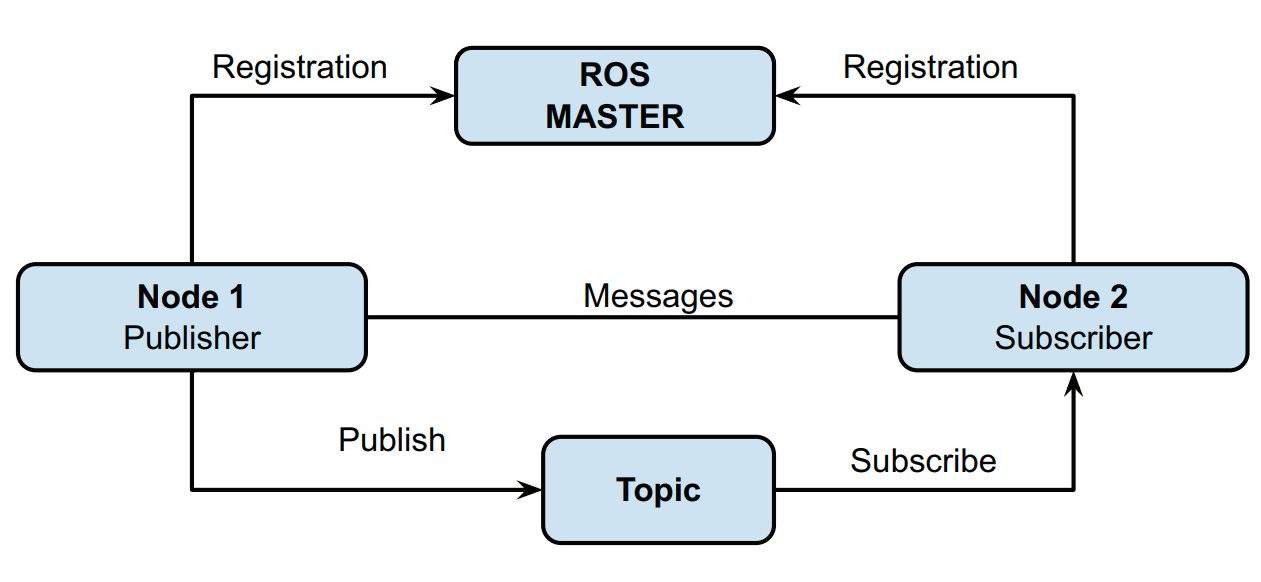
\includegraphics[scale=0.15]{ros-arch.png} % Find the solution of size its creating error 
    \caption{ROS Architecture}
    \label{Fig:ROS Architecture}
\end{figure}

\subsubsection{Gazebo}
The gazebo is a 3D simulation platform that provides robots, sensors, and environment models which are required for robot development. It uses Open Dynamics Engine (ODE) for real-time simulations and graphics. Gazebo supports a wide range of sensors such as LRF,2D/3D camera, Depth Camera, and Force-Torque Sensor. APIs provided in Gazebo enable users to create robots, sensors, and environment control as a plug-in.

\subsubsection{Falcon Haptic Controller}
We are using Novint Falcon as an input for Human-in-the-loop simulation.The Novint Falcon is a haptic device that is designed to provide users with the ability to touch and feel virtual objects in a computer-generated environment. It is typically used in gaming, virtual reality, and simulation applications.The Novint Falcon uses a series of motors and linkages to create force feedback and motion, allowing users to experience the sensation of touch and motion in virtual environments. It has three degrees of freedom (DOF), allowing it to move in the x, y, and z axes. It also has a number of buttons and controls that can be used to interact with the virtual environment.

One of the unique features of the Novint Falcon is its ability to create a wide range of haptic sensations, including force feedback, vibrations, and thermal effects. This allows it to provide a more immersive and realistic experience for users, making it useful for a variety of applications, including gaming, training, and simulation.
\begin{figure}[!ht]
    \centering
    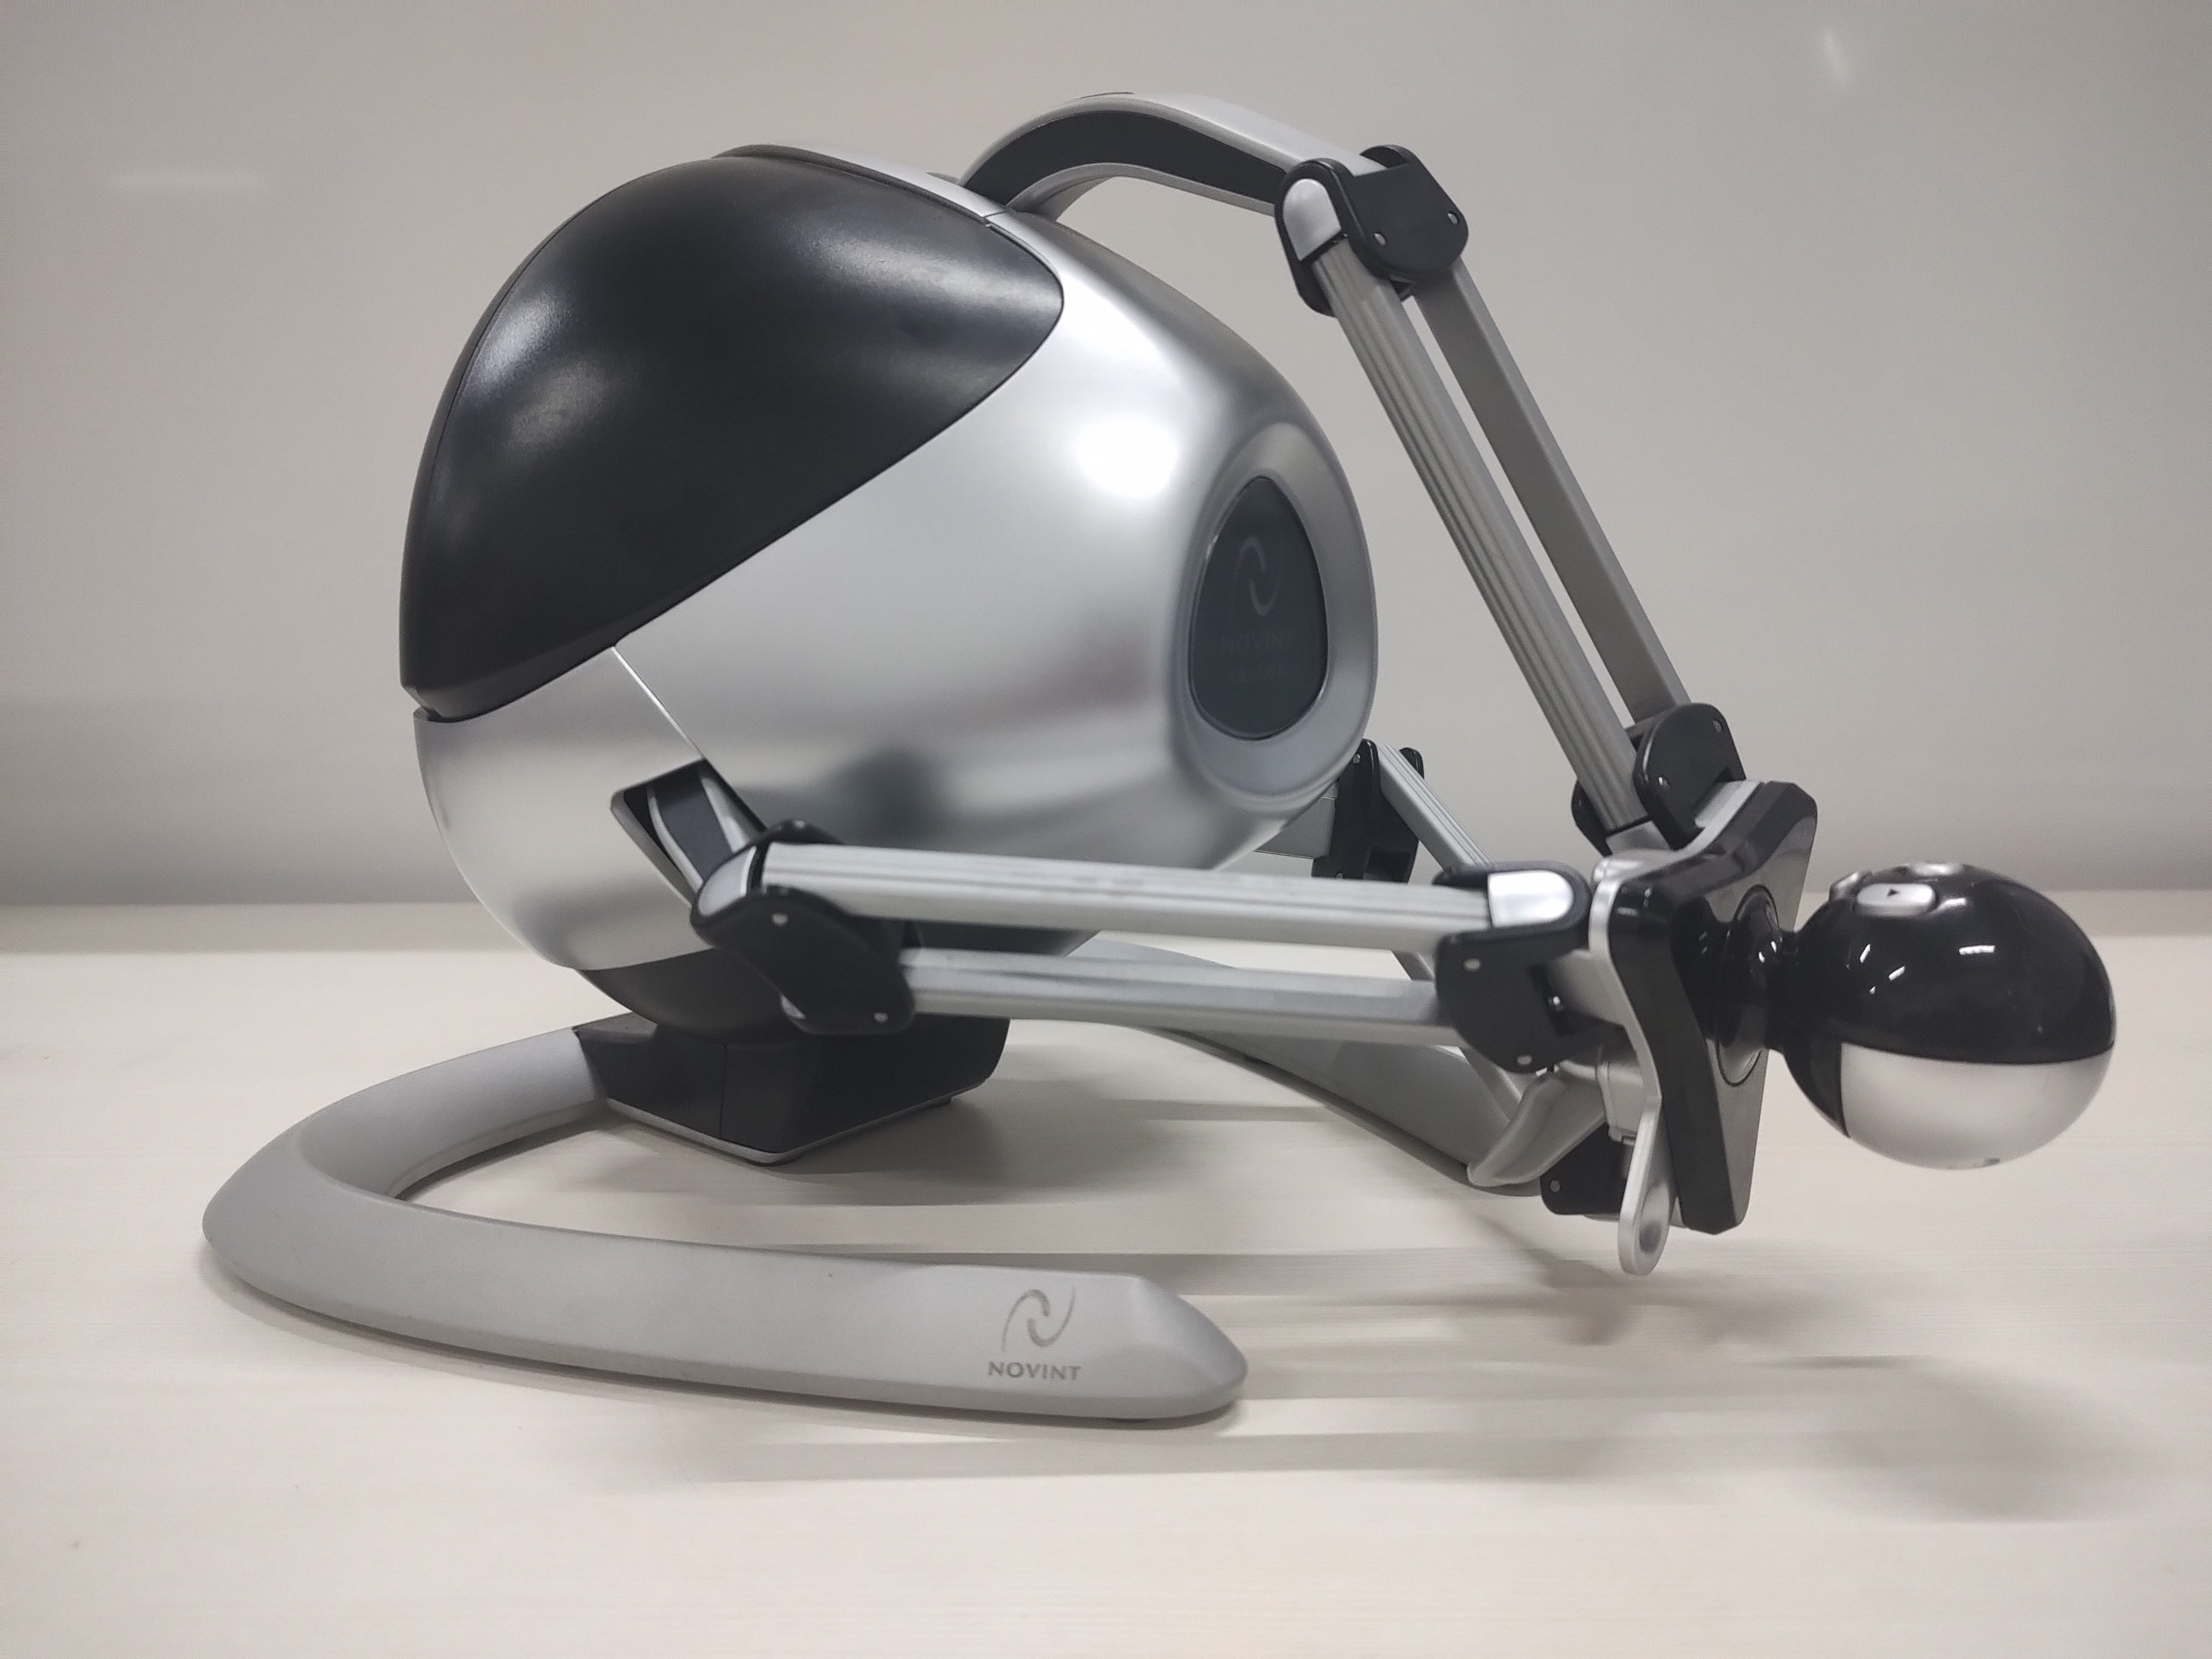
\includegraphics[scale=0.05]{falcon.jpg} % Find the solution of size its creating error 
    \caption{Falcon Haptic Controller}
    \label{Fig:Falcon Haptic Controller}
\end{figure}
Overall, the Novint Falcon is a powerful haptic device that allows users to touch and feel virtual objects in a computer-generated environment, providing a more immersive and realistic experience. It is useful for a variety of applications, including gaming, training, and simulation, and its ability to create a wide range of haptic sensations makes it particularly useful for creating more realistic and engaging virtual environments.
\subsubsection{Crazyflie Quadcopter}
The harware quadcopter used in the testbed for hybrid simulation is Crazyflie 2.1. The Crazyflie 2.1 is a small and lightweight drone developed by Bitcraze, a Swedish robotics company. The Crazyflie 2.1 is equipped with a number of sensors and features that allow it to navigate and stabilize itself in flight. It has an onboard camera, gyroscopes, accelerometers, and magnetometers, as well as a barometer and ultrasound rangefinder. It also has a wireless communication system, allowing it to be controlled remotely using a radio controller or a computer.The Crazyflie 2.1 quadcopter measures 92 millimeters between diagonally opposed motor shafts and weighs 27 grams with a battery. It contains a 32-bit, 168- MHz ARM microcontroller with floating-point unit that is capable of significant onboard computation. Software and hardware are both open-source. The Crazyflie communicates with a PC over the Crazyradio PA, a 2.4 GHz USB radio that transmits up to two megabits per second in 32-byte packets.
\begin{figure}[!ht]
    \centering
        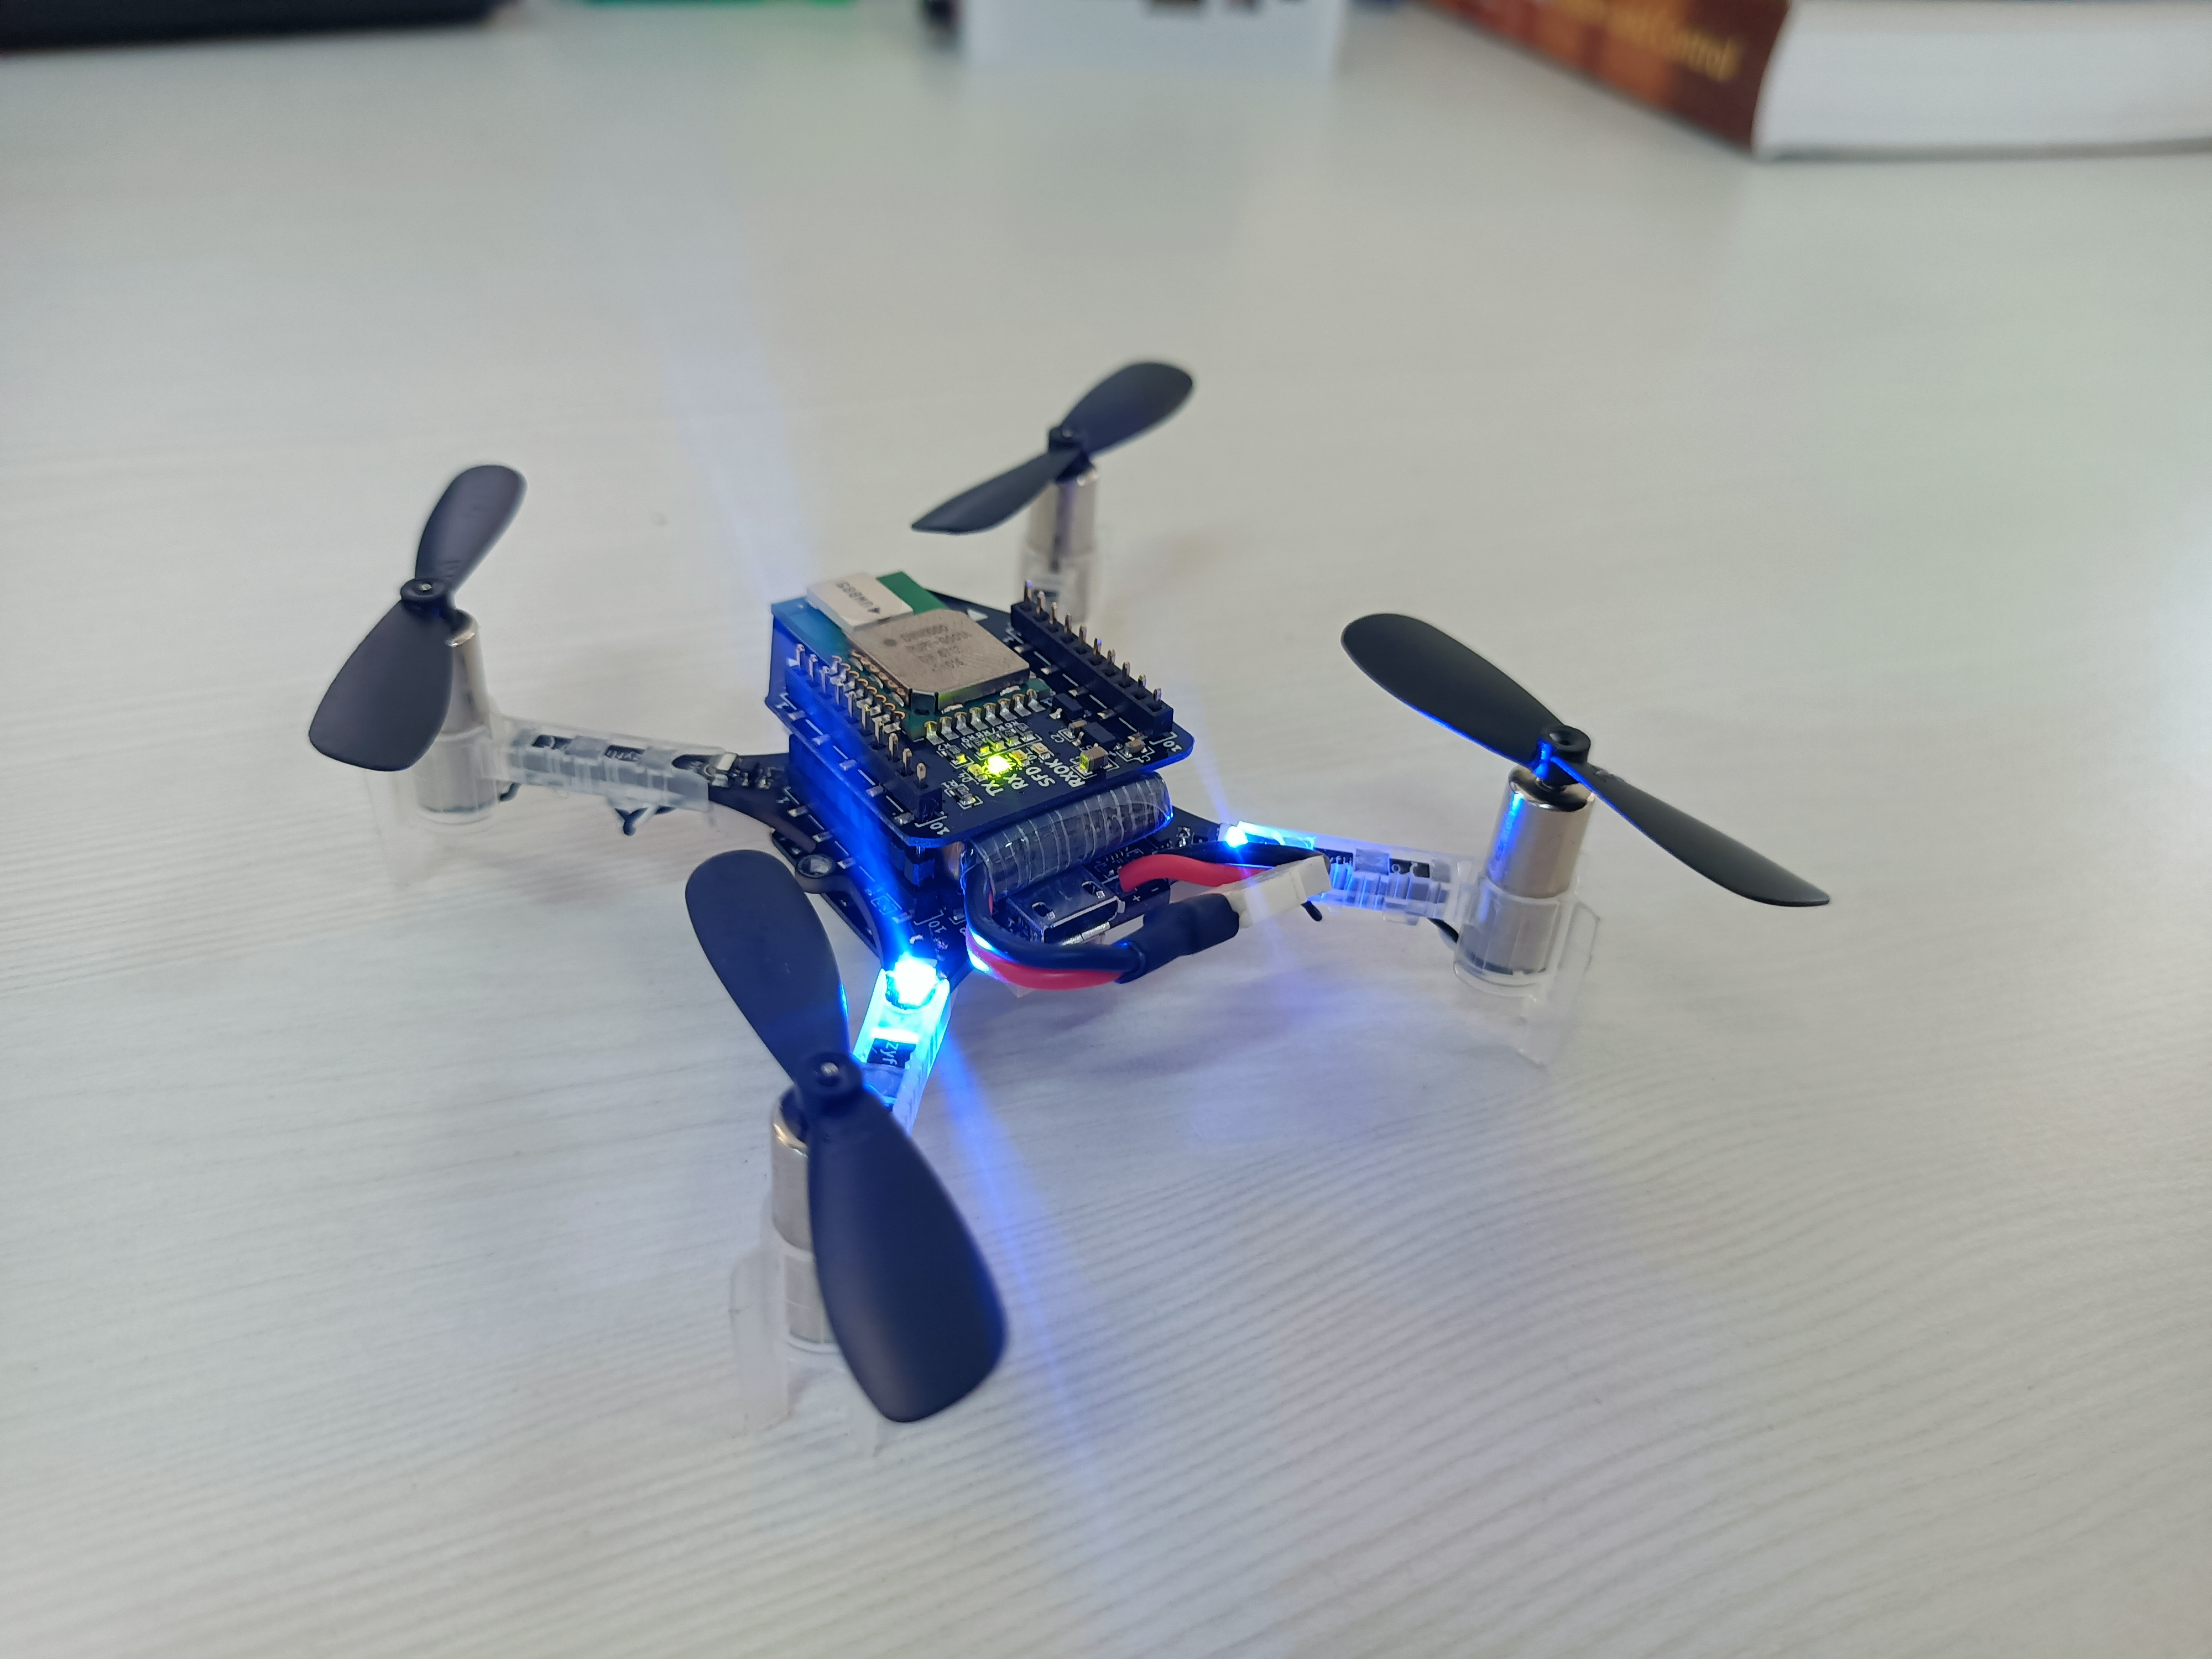
\includegraphics[scale=0.06]{crazyflie.jpg} % Find the solution of size its creating error 
        \caption{Crazyflie Quadcopter}
        \label{Fig:crazyflie}
    \end{figure}
The Crazyflie 2.1 is capable of flying for up to 7 minutes on a single battery charge, and can reach speeds of up to 10 meters per second. It is small and lightweight, weighing just 27 grams, and is capable of flying indoors and outdoors. We have added Optitrack markers and flow deck which increases its weight to 33 grams and reduces the flight time to 6 minutes.\cite{crazyflie}
\subsubsection{Optitrack Localization System}


\subsubsection{Quadcopter Simulation Package}
The quadcopter model used in MASCOT is based on the tum-simulator AR Parrot Drone Gazebo simulation package \cite{Tum} developed by the Computer Vision Group at the Technical University of Munich. The lower level controller is modified and tuned so that the quadcopters can be treated as a double integrator system for control algorithm implementation, and added topics and controls required for the implemented model. A general control script is written for the implementation of the different use cases discussed in Section \ref{sec: Use Cases};





\subsection{Control Block}

\subsubsection{Heading Control}

\subsubsection{Position Control}


\subsection{Architecture and Features of MASCOT}

\subsection{Configuring the Simulation}

\subsection{Configuring the Hybrid - Simulation}


%---------------------- Results ------------------------------------------------

\section{Examples}\label{sec: Use Cases}



\subsection{Simulation with HITL}

\subsubsection{Waypoint Navigation}
\subsubsection{Consensus Algorithms}
\subsubsection{Min-max time Consensus Control}
\subsubsection{Formation Control}

\subsection{Hybrid Simulation with HITL}

\subsubsection{Waypoint Navigation}
\subsubsection{Consensus Algorithms}
\subsubsection{Min-max time Consensus Control}
\subsubsection{Formation Control}

%---------------------- Conclusions ----------------------------------------------

\section{Conclusion and Future Work} \label{sec:conc}



% \begin{IEEEbiography}{Michael Shell}
% Biography text here.
% \end{IEEEbiography}

\bibliographystyle{IEEEtran}
\bibliography{IEEEabrv,references}

\end{document}


